\documentclass[12pt,a4paper]{amsart}
\usepackage[utf8]{inputenc}
\usepackage[T1]{fontenc}
\usepackage{amsmath,amsfonts,amssymb}
\usepackage{tikz}
\usepackage{algorithm}
\usepackage{algorithmic}
\usepackage{float}
\usepackage{listings}
\usepackage{xcolor}
\usepackage{geometry}
\usepackage{fancyhdr}
\usepackage{enumitem}
\usepackage{booktabs}
\usepackage{multirow}
\usepackage[hidelinks,bookmarksnumbered,bookmarksopen]{hyperref}
\usepackage{xeCJK}
\setCJKmainfont{LXGW WenKai}

\geometry{left=2.5cm,right=2.5cm,top=2.5cm,bottom=2.5cm}

% 代码高亮设置
\lstset{
    language=C++,
    basicstyle=\ttfamily\small,
    keywordstyle=\color{blue}\bfseries,
    commentstyle=\color{green!60!black},
    stringstyle=\color{red},
    numbers=left,
    numberstyle=\tiny\color{gray},
    stepnumber=1,
    numbersep=10pt,
    backgroundcolor=\color{gray!10},
    frame=single,
    tabsize=4,
    captionpos=b,
    breaklines=true,
    breakatwhitespace=false,
    showspaces=false,
    showstringspaces=false,
    showtabs=false
}

% 定理环境
\newtheorem{definition}{定义}[section]
\newtheorem{theorem}{定理}[section]

\newtheorem{example}{例题}[section]
\newtheorem{property}{性质}[section]

% TikZ库
\usetikzlibrary{trees,positioning,arrows,automata,calc}

\title{\textbf{数据结构 - 二叉树复习资料}}
\author{详细版本}
\date{\today}

\begin{document}

% \maketitle

% % 目录设置
% \tableofcontents
% \newpage

\section{二叉树的基本概念}

\subsection{树和二叉树的定义}

\begin{definition}[树]
树是$n(n \geq 0)$个结点的有限集合。当$n=0$时,称为空树;任意一棵非空树满足以下条件:
\begin{enumerate}
\item 有且仅有一个特定的称为根的结点;
\item 当$n>1$时,除根结点之外的其余结点被分成$m(m>0)$个互不相交的有限集合$T_1, T_2, \ldots, T_m$,其中每个集合又是一棵树,并称为这个根结点的子树。
\end{enumerate}
\end{definition}

\begin{definition}[二叉树]
二叉树是$n(n \geq 0)$个结点的有限集合,该集合或者为空集(称为空二叉树),或者由一个根结点和两棵互不相交的、分别称为根结点的左子树和右子树的二叉树组成。
\end{definition}

\subsection{二叉树的特点}

二叉树具有以下特点:
\begin{enumerate}
\item 每个结点最多有两棵子树,所以二叉树中不存在度大于2的结点;
\item 二叉树的左右子树不能任意颠倒,如果某结点只有一棵子树,一定要指明它是左子树还是右子树。
\end{enumerate}

\subsection{特殊的二叉树}

\begin{definition}[满二叉树]
在一棵二叉树中,如果所有分支结点都存在左子树和右子树,并且所有叶子都在同一层上,这样的二叉树称为满二叉树。
\end{definition}

\begin{definition}[完全二叉树]
对一棵具有$n$个结点的二叉树按层序编号,如果编号为$i(1 \leq i \leq n)$的结点与同样深度的满二叉树中编号为$i$的结点在二叉树中的位置完全相同,则这棵二叉树称为完全二叉树。
\end{definition}

\begin{center}
\begin{tikzpicture}[level distance=1.5cm,
level 1/.style={sibling distance=4cm},
level 2/.style={sibling distance=2cm},
level 3/.style={sibling distance=1.5cm}]

% 满二叉树示例
\node at (-4,3) {\textbf{满二叉树}};
\node[circle,draw] at (-4,2) {1}
    child {node[circle,draw] {2}
        child {node[circle,draw] {4}}
        child {node[circle,draw] {5}}}
    child {node[circle,draw] {3}
        child {node[circle,draw] {6}}
        child {node[circle,draw] {7}}};

% 完全二叉树示例
\node at (4,3) {\textbf{完全二叉树}};
\node[circle,draw] at (4,2) {1}
    child {node[circle,draw] {2}
        child {node[circle,draw] {4}}
        child {node[circle,draw] {5}}}
    child {node[circle,draw] {3}
        child {node[circle,draw] {6}}
        child[missing]};
\end{tikzpicture}
\end{center}

\section{二叉树的基本性质}

\begin{property}[性质1]
在一棵二叉树中,如果叶子结点的个数为$n_0$,度为2的结点个数为$n_2$,则$n_0 = n_2 + 1$。
\end{property}

\begin{proof}
设二叉树的结点总数为$N$,叶子结点(度为0)的个数为$n_0$,度为1的结点个数为$n_1$,度为2的结点个数为$n_2$。
根据定义,树中任意一个结点,其度数(即子结点数)只能是0, 1或2。因此,结点总数可以表示为:
$$N = n_0 + n_1 + n_2 \quad (1)$$

现在,我们从两个不同的角度来考虑树中的分枝(边)的总数,设为$B$。

\textbf{角度一:从结点与边的关系来看}
对于一棵非空树,除了根结点,每个结点都有且仅有一个父结点,对应一条进入该结点的分枝。因此,分枝总数等于结点总数减1。
$$B = N - 1 \quad (2)$$

\textbf{角度二:从结点度数与边的关系来看}
树中所有分枝都是由度为1或度为2的结点发出的。每个度为1的结点发出一条分枝,每个度为2的结点发出两条分枝。因此,分枝总数等于所有结点的度数之和。
$$B = (0 \cdot n_0) + (1 \cdot n_1) + (2 \cdot n_2) = n_1 + 2n_2 \quad (3)$$

联立等式 (2) 和 (3),我们得到:
$$N - 1 = n_1 + 2n_2$$
将等式 (1) 代入上式,用 $n_0 + n_1 + n_2$ 替换 $N$:
$$(n_0 + n_1 + n_2) - 1 = n_1 + 2n_2$$
对上式进行化简,两边同时减去 $n_1$:
$$n_0 + n_2 - 1 = 2n_2$$
两边再同时减去 $n_2$:
$$n_0 - 1 = n_2$$
最终得到:
$$n_0 = n_2 + 1$$
此性质对于空树也成立(此时 $n_0=0, n_2=0$)。
\end{proof}

\begin{property}[性质2]
二叉树的第$i$层上最多有$2^{i-1}$个结点$(i \geq 1)$。
\end{property}

\begin{property}[性质3]
在一棵深度为$k$的二叉树中,最多有$2^k - 1$个结点。
\end{property}

\begin{property}[性质4]
具有$n$个结点的完全二叉树的深度为$\lfloor\log_2 n\rfloor + 1$。
\end{property}

\begin{property}[性质5]
对一棵具有$n$个结点的完全二叉树从1开始按层序编号,则对于编号为$i(1 \leq i \leq n)$的结点,有如下关系成立:
\begin{enumerate}
\item 如果$i > 1$,则结点$i$的双亲的编号为$\lfloor i/2 \rfloor$;否则结点$i$是根结点,无双亲。
\item 如果$2i \leq n$,则结点$i$的左孩子的编号为$2i$;否则结点$i$无左孩子。
\item 如果$2i+1 \leq n$,则结点$i$的右孩子的编号为$2i+1$;否则结点$i$无右孩子。
\end{enumerate}
\end{property}

\section{二叉树的存储结构}

\subsection{顺序存储结构}

二叉树的顺序存储结构是用一维数组存储二叉树的结点,用结点的存储位置(下标)表示结点之间的逻辑关系。

\begin{center}
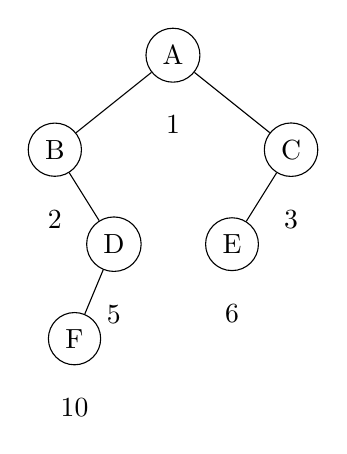
\begin{tikzpicture}[level distance=1.2cm,
level 1/.style={sibling distance=3cm},
level 2/.style={sibling distance=1.5cm},
level 3/.style={sibling distance=1cm}]

\node[circle,draw] (1) {A}
    child {node[circle,draw] (2) {B}
        child[missing]
        child {node[circle,draw] (5) {D}
            child {node[circle,draw] (10) {F}}
            child[missing]}}
    child {node[circle,draw] (3) {C}
        child {node[circle,draw] (6) {E}}
        child[missing]};

% 添加编号
\node[below=0.3cm of 1] {1};
\node[below=0.3cm of 2] {2};
\node[below=0.3cm of 3] {3};
\node[below=0.3cm of 5] {5};
\node[below=0.3cm of 6] {6};
\node[below=0.3cm of 10] {10};
\end{tikzpicture}
\end{center}

顺序存储数组:
\begin{center}
\begin{tabular}{|c|c|c|c|c|c|c|c|c|c|c|}
\hline
下标 & 1 & 2 & 3 & 4 & 5 & 6 & 7 & 8 & 9 & 10 \\
\hline
元素 & A & B & C & $\emptyset$ & D & E & $\emptyset$ & $\emptyset$ & $\emptyset$ & F \\
\hline
\end{tabular}
\end{center}

\subsection{二叉链表}

二叉链表的结点结构:
\begin{center}
\begin{tabular}{|c|c|c|}
\hline
lchild & data & rchild \\
\hline
\end{tabular}
\end{center}

\begin{lstlisting}[caption=二叉链表结点定义]
template <typename DataType>
struct BiNode {
    DataType data;
    BiNode<DataType> *lchild, *rchild;
};
\end{lstlisting}

\section{二叉树的遍历}

\subsection{遍历方法}

二叉树的遍历是指从根结点出发,按照某种次序访问二叉树中的所有结点,使得每个结点被访问一次且仅被访问一次。

\begin{definition}[前序遍历]
若二叉树为空,则空操作返回;否则执行下述操作:
\begin{enumerate}
\item 访问根结点;
\item 前序遍历根结点的左子树;
\item 前序遍历根结点的右子树。
\end{enumerate}
\end{definition}

\begin{definition}[中序遍历]
若二叉树为空,则空操作返回;否则执行下述操作:
\begin{enumerate}
\item 中序遍历根结点的左子树;
\item 访问根结点;
\item 中序遍历根结点的右子树。
\end{enumerate}
\end{definition}

\begin{definition}[后序遍历]
若二叉树为空,则空操作返回;否则执行下述操作:
\begin{enumerate}
\item 后序遍历根结点的左子树;
\item 后序遍历根结点的右子树;
\item 访问根结点。
\end{enumerate}
\end{definition}

\begin{definition}[层序遍历]
从二叉树的根结点开始,从上至下逐层遍历,同一层按从左到右的顺序对结点逐个访问。
\end{definition}

\subsection{遍历算法实现}

\noindent

\begin{algorithm}[H]
\caption{前序遍历递归算法}
\begin{algorithmic}[1]
\REQUIRE 二叉树根指针$bt$
\ENSURE 输出前序遍历序列
\IF{$bt \neq NULL$}
\STATE 访问$bt$的数据域
\STATE 前序遍历$bt$的左子树
\STATE 前序遍历$bt$的右子树
\ENDIF
\end{algorithmic}
\end{algorithm}

\begin{lstlisting}[caption=前序遍历递归实现]
template <typename DataType>
void PreOrder(BiNode<DataType> *bt) {
    if (bt == nullptr) return;
    cout << bt->data << "\t";    // 访问根结点
    PreOrder(bt->lchild);        // 遍历左子树
    PreOrder(bt->rchild);        // 遍历右子树
}
\end{lstlisting}

\begin{example}[前序遍历示例]
给定如下二叉树:
\begin{center}
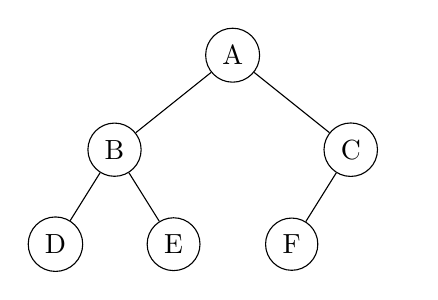
\begin{tikzpicture}[level distance=1.2cm,
    level 1/.style={sibling distance=3cm},
    level 2/.style={sibling distance=1.5cm},
    level 3/.style={sibling distance=1cm}]
\node[circle,draw] {A}
    child {node[circle,draw] {B}
        child {node[circle,draw] {D}}
        child {node[circle,draw] {E}}
    }
    child {node[circle,draw] {C}
        child {node[circle,draw] {F}}
        child {edge from parent[draw=none]}
    };
\end{tikzpicture}
\end{center}

前序遍历过程:
\begin{enumerate}
\item 访问根结点A,输出A
\item 前序遍历左子树(以B为根):
    \begin{itemize}
    \item 访问B,输出B
    \item 前序遍历B的左子树:访问D,输出D
    \item 前序遍历B的右子树:访问E,输出E
    \end{itemize}
\item 前序遍历右子树(以C为根):
    \begin{itemize}
    \item 访问C,输出C
    \item 前序遍历C的左子树:访问F,输出F
    \item 前序遍历C的右子树:空
    \end{itemize}
\end{enumerate}

\textbf{前序遍历结果:A B D E C F}
\end{example}

\begin{algorithm}[H]
\caption{中序遍历递归算法}
\begin{algorithmic}[1]
\REQUIRE 二叉树根指针$bt$
\ENSURE 输出中序遍历序列
\IF{$bt \neq NULL$}
\STATE 中序遍历$bt$的左子树
\STATE 访问$bt$的数据域
\STATE 中序遍历$bt$的右子树
\ENDIF
\end{algorithmic}
\end{algorithm}

\begin{lstlisting}[caption=中序遍历递归实现]
template <typename DataType>
void InOrder(BiNode<DataType> *bt) {
    if (bt == nullptr) return;
    InOrder(bt->lchild);         // 遍历左子树
    cout << bt->data << "\t";    // 访问根结点
    InOrder(bt->rchild);         // 遍历右子树
}
\end{lstlisting}
\begin{center}
    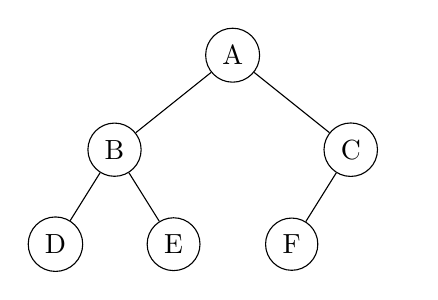
\begin{tikzpicture}[level distance=1.2cm,
        level 1/.style={sibling distance=3cm},
        level 2/.style={sibling distance=1.5cm},
        level 3/.style={sibling distance=1cm}]
    \node[circle,draw] {A}
        child {node[circle,draw] {B}
            child {node[circle,draw] {D}}
            child {node[circle,draw] {E}}
        }
        child {node[circle,draw] {C}
            child {node[circle,draw] {F}}
            child {edge from parent[draw=none]}
        };
    \end{tikzpicture}
    \end{center}
\begin{example}[中序遍历示例]
使用同一棵二叉树,中序遍历过程:
\begin{enumerate}
\item 中序遍历左子树(以B为根):
    \begin{itemize}
    \item 中序遍历B的左子树:访问D,输出D
    \item 访问B,输出B
    \item 中序遍历B的右子树:访问E,输出E
    \end{itemize}
\item 访问根结点A,输出A
\item 中序遍历右子树(以C为根):
    \begin{itemize}
    \item 中序遍历C的左子树:访问F,输出F
    \item 访问C,输出C
    \item 中序遍历C的右子树:空
    \end{itemize}
\end{enumerate}

\textbf{中序遍历结果:D B E A F C}
\end{example}

\begin{algorithm}[H]
\caption{后序遍历递归算法}
\begin{algorithmic}[1]
\REQUIRE 二叉树根指针$bt$
\ENSURE 输出后序遍历序列
\IF{$bt \neq NULL$}
\STATE 后序遍历$bt$的左子树
\STATE 后序遍历$bt$的右子树
\STATE 访问$bt$的数据域
\ENDIF
\end{algorithmic}
\end{algorithm}

\begin{lstlisting}[caption=后序遍历递归实现]
template <typename DataType>
void PostOrder(BiNode<DataType> *bt) {
    if (bt == nullptr) return;
    PostOrder(bt->lchild);       // 遍历左子树
    PostOrder(bt->rchild);       // 遍历右子树
    cout << bt->data << "\t";    // 访问根结点
}
\end{lstlisting}
\begin{center}
    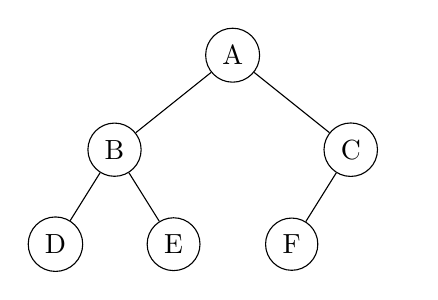
\begin{tikzpicture}[level distance=1.2cm,
        level 1/.style={sibling distance=3cm},
        level 2/.style={sibling distance=1.5cm},
        level 3/.style={sibling distance=1cm}]
    \node[circle,draw] {A}
        child {node[circle,draw] {B}
            child {node[circle,draw] {D}}
            child {node[circle,draw] {E}}
        }
        child {node[circle,draw] {C}
            child {node[circle,draw] {F}}
            child {edge from parent[draw=none]}
        };
    \end{tikzpicture}
    \end{center}
\begin{example}[后序遍历示例]
使用同一棵二叉树,后序遍历过程:
\begin{enumerate}
\item 后序遍历左子树(以B为根):
    \begin{itemize}
    \item 后序遍历B的左子树:访问D,输出D
    \item 后序遍历B的右子树:访问E,输出E
    \item 访问B,输出B
    \end{itemize}
\item 后序遍历右子树(以C为根):
    \begin{itemize}
    \item 后序遍历C的左子树:访问F,输出F
    \item 后序遍历C的右子树:空
    \item 访问C,输出C
    \end{itemize}
\item 访问根结点A,输出A
\end{enumerate}

\textbf{后序遍历结果:D E B F C A}
\end{example}

\begin{example}[更复杂的遍历示例]
考虑一个更复杂的二叉树:
\begin{center}
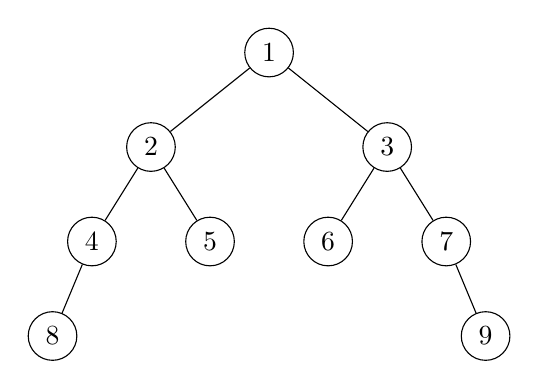
\begin{tikzpicture}[level distance=1.2cm,
    level 1/.style={sibling distance=3cm},
    level 2/.style={sibling distance=1.5cm},
    level 3/.style={sibling distance=1cm}]
\node[circle,draw] {1}
    child {node[circle,draw] {2}
        child {node[circle,draw] {4}
            child {node[circle,draw] {8}}
            child[missing]
        }
        child {node[circle,draw] {5}}
    }
    child {node[circle,draw] {3}
        child {node[circle,draw] {6}}
        child {node[circle,draw] {7}
            child[missing]
            child {node[circle,draw] {9}}
        }
    };
\end{tikzpicture}
\end{center}

\textbf{三种遍历结果比较:}
\begin{itemize}
\item \textbf{前序遍历:}1 2 4 8 5 3 6 7 9
\item \textbf{中序遍历:}8 4 2 5 1 6 3 7 9
\item \textbf{后序遍历:}8 4 5 2 6 9 7 3 1
\end{itemize}

\textbf{规律总结:}
\begin{itemize}
\item 前序遍历:根结点总是在对应子树的最前面
\item 中序遍历:根结点总是在其左右子树之间
\item 后序遍历:根结点总是在对应子树的最后面
\end{itemize}
\end{example}

\subsection{非递归遍历算法}

\indent

\begin{algorithm}[H]
\caption{前序遍历非递归算法}
\begin{algorithmic}[1]
\REQUIRE 二叉树根指针$bt$
\ENSURE 输出前序遍历序列
\STATE 初始化栈$S$
\IF{二叉树非空}
    \STATE 将根指针$bt$入栈
    \WHILE{栈$S$不为空}
        \STATE $p \leftarrow$ 栈顶元素出栈
        \STATE 访问结点$p$的数据域
        \IF{结点$p$存在右孩子}
            \STATE 将右孩子指针入栈
        \ENDIF
        \IF{结点$p$存在左孩子}
            \STATE 将左孩子指针入栈
        \ENDIF
    \ENDWHILE
\ENDIF
\end{algorithmic}
\end{algorithm}

\begin{lstlisting}[caption=前序遍历非递归实现]
template <typename DataType>
void PreOrderNonRecur(BiNode<DataType> *bt) {
    if (bt == nullptr) return;
    stack<BiNode<DataType>*> S;
    S.push(bt);
    
    while (!S.empty()) {
        BiNode<DataType> *p = S.top();
        S.pop();
        cout << p->data << "\t";    // 访问结点
        
        if (p->rchild != nullptr)   // 右孩子先入栈
            S.push(p->rchild);
        if (p->lchild != nullptr)   // 左孩子后入栈(先出栈)
            S.push(p->lchild);
    }
}
\end{lstlisting}

\begin{algorithm}[H]
\caption{中序遍历非递归算法}
\begin{algorithmic}[1]
\REQUIRE 二叉树根指针$bt$
\ENSURE 输出中序遍历序列
\STATE 初始化栈$S$
\STATE $p \leftarrow bt$
\WHILE{$p \neq NULL$ OR 栈$S$不为空}
    \WHILE{$p \neq NULL$}
        \STATE 将$p$入栈
        \STATE $p \leftarrow p$的左孩子
    \ENDWHILE
    \IF{栈$S$不为空}
        \STATE $p \leftarrow$ 栈顶元素出栈
        \STATE 访问结点$p$的数据域
        \STATE $p \leftarrow p$的右孩子
    \ENDIF
\ENDWHILE
\end{algorithmic}
\end{algorithm}

\begin{lstlisting}[caption=中序遍历非递归实现]
template <typename DataType>
void InOrderNonRecur(BiNode<DataType> *bt) {
    stack<BiNode<DataType>*> S;
    BiNode<DataType> *p = bt;
    
    while (p != nullptr || !S.empty()) {
        while (p != nullptr) {      // 一直向左走到底
            S.push(p);
            p = p->lchild;
        }
        if (!S.empty()) {
            p = S.top();
            S.pop();
            cout << p->data << "\t";    // 访问结点
            p = p->rchild;              // 转向右子树
        }
    }
}
\end{lstlisting}

\begin{algorithm}[H]
\caption{后序遍历非递归算法}
\begin{algorithmic}[1]
\REQUIRE 二叉树根指针$bt$
\ENSURE 输出后序遍历序列
\STATE 初始化栈$S$
\STATE $p \leftarrow bt$, $r \leftarrow NULL$
\WHILE{$p \neq NULL$ OR 栈$S$不为空}
    \IF{$p \neq NULL$}
        \STATE 将$p$入栈
        \STATE $p \leftarrow p$的左孩子
    \ELSE
        \STATE $p \leftarrow$ 栈顶元素(不出栈)
        \IF{$p$的右孩子存在且$p$的右孩子$\neq r$}
            \STATE $p \leftarrow p$的右孩子
        \ELSE
            \STATE $p \leftarrow$ 栈顶元素出栈
            \STATE 访问结点$p$的数据域
            \STATE $r \leftarrow p$
            \STATE $p \leftarrow NULL$
        \ENDIF
    \ENDIF
\ENDWHILE
\end{algorithmic}
\end{algorithm}

\begin{lstlisting}[caption=后序遍历非递归实现]
template <typename DataType>
void PostOrderNonRecur(BiNode<DataType> *bt) {
    if (bt == nullptr) return;
    stack<BiNode<DataType>*> S;
    BiNode<DataType> *p = bt;
    BiNode<DataType> *r = nullptr;  // 标记最近访问过的结点
    
    while (p != nullptr || !S.empty()) {
        if (p != nullptr) {         // 走到最左边
            S.push(p);
            p = p->lchild;
        } else {
            p = S.top();            // 查看栈顶元素
            if (p->rchild != nullptr && p->rchild != r) {
                p = p->rchild;      // 转向右子树
            } else {
                p = S.top();
                S.pop();
                cout << p->data << "\t";  // 访问结点
                r = p;              // 记录最近访问的结点
                p = nullptr;        // 结点访问完后,重置p指针
            }
        }
    }
}
\end{lstlisting}

\begin{algorithm}[H]
\caption{层序遍历算法}
\begin{algorithmic}[1]
\REQUIRE 二叉树根指针$bt$
\ENSURE 输出层序遍历序列
\STATE 初始化队列$Q$
\IF{二叉树非空}
    \STATE 将根指针入队
    \WHILE{队列$Q$不为空}
        \STATE $q \leftarrow$ 队头元素出队
        \STATE 访问结点$q$的数据域
        \IF{结点$q$存在左孩子}
            \STATE 将左孩子指针入队
        \ENDIF
        \IF{结点$q$存在右孩子}
            \STATE 将右孩子指针入队
        \ENDIF
    \ENDWHILE
\ENDIF
\end{algorithmic}
\end{algorithm}

\begin{lstlisting}[caption=层序遍历实现]
template <typename DataType>
void LevelOrder(BiNode<DataType> *bt) {
    if (bt == nullptr) return;
    queue<BiNode<DataType>*> Q;
    Q.push(bt);
    
    while (!Q.empty()) {
        BiNode<DataType> *q = Q.front();
        Q.pop();
        cout << q->data << "\t";    // 访问结点
        
        if (q->lchild != nullptr)   // 左孩子入队
            Q.push(q->lchild);
        if (q->rchild != nullptr)   // 右孩子入队
            Q.push(q->rchild);
    }
}
\end{lstlisting}

\subsection{遍历算法复杂度分析}

\begin{theorem}[遍历算法时间复杂度]
对于具有$n$个结点的二叉树:
\begin{itemize}
\item 递归遍历算法的时间复杂度均为$O(n)$,空间复杂度为$O(h)$,其中$h$为树的高度
\item 非递归遍历算法的时间复杂度均为$O(n)$,空间复杂度为$O(h)$
\item 层序遍历算法的时间复杂度为$O(n)$,空间复杂度为$O(w)$,其中$w$为树的最大宽度
\end{itemize}
\end{theorem}

\subsection{遍历示例}

\begin{center}
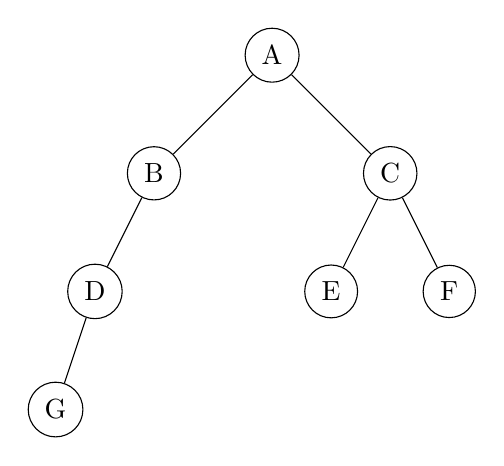
\begin{tikzpicture}[level distance=1.5cm,
level 1/.style={sibling distance=3cm},
level 2/.style={sibling distance=1.5cm},
level 3/.style={sibling distance=1cm}]

\node[circle,draw] {A}
    child {node[circle,draw] {B}
        child {node[circle,draw] {D}
            child {node[circle,draw] {G}}
            child[missing]}
        child[missing]}
    child {node[circle,draw] {C}
        child {node[circle,draw] {E}}
        child {node[circle,draw] {F}}};
\end{tikzpicture}
\end{center}

对于上述二叉树,各种遍历序列为:
\begin{itemize}
\item 前序遍历:A B D G C E F
\item 中序遍历:G D B A E C F
\item 后序遍历:G D B E F C A
\item 层序遍历:A B C D E F G
\end{itemize}

\section{二叉树的构造}

\begin{theorem}
前序遍历序列和中序遍历序列能唯一确定一棵二叉树。
\end{theorem}

\begin{example}[由遍历序列构造二叉树]
已知一棵二叉树的前序遍历序列为ABDCEF,中序遍历序列为DBAECF,构造该二叉树。

\textbf{解:}
\begin{enumerate}
\item 由前序序列可知,A是二叉树的根结点。
\item 根据中序序列,在A之前的所有结点(DB)都是A的左子树的结点,在A之后的所有结点(ECF)都是A的右子树的结点。
\item 对左子树:前序序列为BD,中序序列为DB。由前序序列知B是左子树的根结点,由中序序列知D是B的左子树结点。
\item 对右子树:前序序列为CEF,中序序列为ECF。由前序序列知C是右子树的根结点,由中序序列知E是C的左子树结点,F是C的右子树结点。
\end{enumerate}

构造过程如下:

\begin{center}
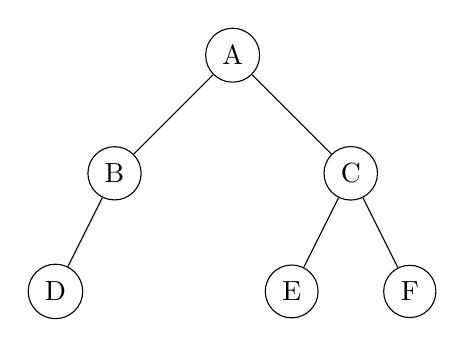
\begin{tikzpicture}[level distance=1.5cm,
level 1/.style={sibling distance=3cm},
level 2/.style={sibling distance=1.5cm}]

\node[circle,draw] {A}
    child {node[circle,draw] {B}
        child {node[circle,draw] {D}}
        child[missing]}
    child {node[circle,draw] {C}
        child {node[circle,draw] {E}}
        child {node[circle,draw] {F}}};
\end{tikzpicture}
\end{center}
\end{example}

\section{线索二叉树}

\subsection{线索二叉树的基本概念}

在具有$n$个结点的二叉链表中,共有$2n$个指针域,其中只有$n-1$个指针域用来存储孩子结点的地址,存在$n+1$个空指针域。可以利用这些空指针指向该结点在某种遍历序列中的前驱和后继结点。

\begin{definition}[线索]
指向前驱和后继结点的指针称为线索。
\end{definition}

\begin{definition}[线索二叉树]
加上线索的二叉树称为线索二叉树。
\end{definition}

\subsection{线索二叉树的结点结构}

\begin{center}
\begin{tabular}{|c|c|c|c|c|}
\hline
lchild & ltag & data & rtag & rchild \\
\hline
\end{tabular}
\end{center}

其中:
$$ltag = \begin{cases}
0 & \text{lchild指向该结点的左孩子} \\
1 & \text{lchild指向该结点的前驱}
\end{cases}$$

$$rtag = \begin{cases}
0 & \text{rchild指向该结点的右孩子} \\
1 & \text{rchild指向该结点的后继}
\end{cases}$$

\begin{lstlisting}[caption=线索二叉树结点定义]
template <typename DataType>
struct ThrNode {
    DataType data;
    int ltag, rtag;
    ThrNode<DataType> *lchild, *rchild;
};
\end{lstlisting}

\section{哈夫曼树}

\subsection{基本概念}

\begin{definition}[权值]
叶子结点的权值是对叶子结点赋予的一个有意义的数值量。
\end{definition}

\begin{definition}[带权路径长度]
设二叉树具有$n$个带权值的叶子结点,从根结点到各个叶子结点的路径长度与相应叶子结点权值的乘积之和称为二叉树的带权路径长度,记为:
$$WPL = \sum_{k=1}^{n} w_k l_k$$
其中,$w_k$为第$k$个叶子结点的权值;$l_k$为从根结点到第$k$个叶子结点的路径长度。
\end{definition}

\begin{definition}[哈夫曼树]
带权路径长度最小的二叉树称为最优二叉树,也称哈夫曼树。
\end{definition}

\subsection{哈夫曼算法}

\begin{algorithm}[H]
\caption{哈夫曼算法}
\begin{algorithmic}[1]
\REQUIRE $n$个权值$\{w_1, w_2, \ldots, w_n\}$
\ENSURE 哈夫曼树
\STATE 初始化:由$\{w_1, w_2, \ldots, w_n\}$构造$n$棵只有一个根结点的二叉树,从而得到一个二叉树集合$F = \{T_1, T_2, \ldots, T_n\}$
\WHILE{集合$F$中的二叉树个数大于1}
    \STATE 选取与合并:在$F$中选取根结点的权值最小的两棵二叉树分别作为左右子树构造一棵新的二叉树,新根结点的权值为其左右子树根结点的权值之和
    \STATE 删除与加入:在$F$中删除作为左右子树的两棵二叉树,并将新建立的二叉树加入到$F$中
\ENDWHILE
\end{algorithmic}
\end{algorithm}

\begin{example}[哈夫曼树构造]
给定权值集合$\{2, 3, 4, 5\}$,构造哈夫曼树。

\textbf{解:}

\begin{center}
\textbf{构造步骤:}

\begin{enumerate}
\item \textbf{初始状态:}四个独立结点,权值分别为2, 3, 4, 5
\item \textbf{第一步:}选择权值最小的两个结点(2和3)进行合并,生成权值为5的新结点
\item \textbf{第二步:}选择权值最小的两个结点(4和5)进行合并,生成权值为9的新结点
\item \textbf{第三步:}最后将两个子树(权值为5和9)合并,生成根结点,权值为14
\end{enumerate}

\textbf{步骤1:初始状态}

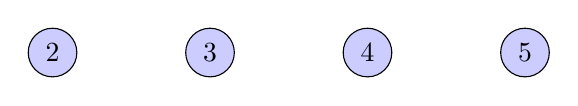
\begin{tikzpicture}
\node[circle,draw,fill=blue!20] at (0,0) {2};
\node[circle,draw,fill=blue!20] at (2,0) {3};
\node[circle,draw,fill=blue!20] at (4,0) {4};
\node[circle,draw,fill=blue!20] at (6,0) {5};
\end{tikzpicture}

\vspace{0.8cm}

\textbf{步骤2:第一次合并(2 + 3 = 5)}

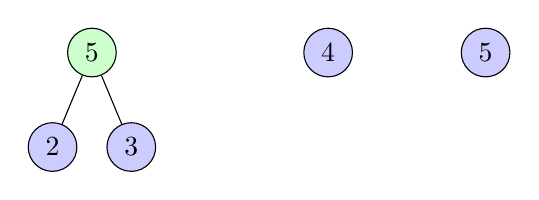
\begin{tikzpicture}[level distance=1.2cm, sibling distance=1cm]
\node[circle,draw,fill=green!20] at (1,0) {5}
    child {node[circle,draw,fill=blue!20] {2}}
    child {node[circle,draw,fill=blue!20] {3}};
\node[circle,draw,fill=blue!20] at (4,0) {4};
\node[circle,draw,fill=blue!20] at (6,0) {5};
\end{tikzpicture}

\vspace{0.8cm}

\textbf{步骤3:第二次合并(4 + 5 = 9)}

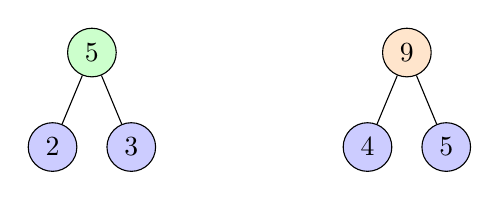
\begin{tikzpicture}[level distance=1.2cm, sibling distance=1cm]
\node[circle,draw,fill=green!20] at (1,0) {5}
    child {node[circle,draw,fill=blue!20] {2}}
    child {node[circle,draw,fill=blue!20] {3}};
\node[circle,draw,fill=orange!20] at (5,0) {9}
    child {node[circle,draw,fill=blue!20] {4}}
    child {node[circle,draw,fill=blue!20] {5}};
\end{tikzpicture}

\vspace{0.8cm}

\textbf{步骤4:最终合并(5 + 9 = 14)}

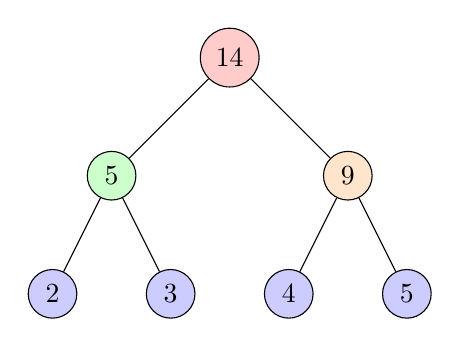
\begin{tikzpicture}[level distance=1.5cm, 
level 1/.style={sibling distance=3cm},
level 2/.style={sibling distance=1.5cm}]
\node[circle,draw,fill=red!20] {14}
    child {node[circle,draw,fill=green!20] {5}
        child {node[circle,draw,fill=blue!20] {2}}
        child {node[circle,draw,fill=blue!20] {3}}}
    child {node[circle,draw,fill=orange!20] {9}
        child {node[circle,draw,fill=blue!20] {4}}
        child {node[circle,draw,fill=blue!20] {5}}};
\end{tikzpicture}
\end{center}
该哈夫曼树的带权路径长度计算如下:

根据带权路径长度公式 $WPL = \sum_{k=1}^{n} w_k l_k$,我们需要计算每个叶子结点的权值乘以其到根结点的路径长度:

\begin{itemize}
\item 权值为2的叶子结点:从根结点到该结点需要经过3条边(根→左子树→左子树→左叶子),所以路径长度$l_1 = 3$
\item 权值为3的叶子结点:从根结点到该结点需要经过3条边(根→左子树→左子树→右叶子),所以路径长度$l_2 = 3$  
\item 权值为4的叶子结点:从根结点到该结点需要经过2条边(根→右子树→左叶子),所以路径长度$l_3 = 2$
\item 权值为5的叶子结点:从根结点到该结点需要经过2条边(根→右子树→右叶子),所以路径长度$l_4 = 2$
\end{itemize}

因此,带权路径长度为:
$$WPL = 2 \times 3 + 3 \times 3 + 4 \times 2 + 5 \times 2 = 6 + 9 + 8 + 10 = 33$$
\end{example}

\subsection{哈夫曼编码}

哈夫曼树可用于构造最短的不等长编码方案:
\begin{enumerate}
\item 以字符作为叶子结点,频率作为权值构造哈夫曼树
\item 规定左分支代表0,右分支代表1
\item 从根结点到叶子结点的路径组成该字符的编码
\end{enumerate}

\begin{example}[哈夫曼编码]
字符集$\{A, B, C, D, E\}$,使用频率分别为$\{35, 25, 15, 15, 10\}$,构造哈夫曼编码。

\textbf{构造步骤:}

\textbf{步骤1:}将所有字符按频率从小到大排列:$E(10), C(15), D(15), B(25), A(35)$

\textbf{步骤2:}选择频率最小的两个结点$E(10)$和$C(15)$合并,得到新结点权值为$10+15=25$

\textbf{步骤3:}选择频率最小的两个结点$D(15)$和新结点$(25)$合并,得到新结点权值为$15+25=40$

\textbf{步骤4:}选择频率最小的两个结点$B(25)$和$A(35)$合并,得到新结点权值为$25+35=60$

\textbf{步骤5:}最后合并剩余的两个结点$(40)$和$(60)$,得到根结点权值为$40+60=100$

\begin{center}
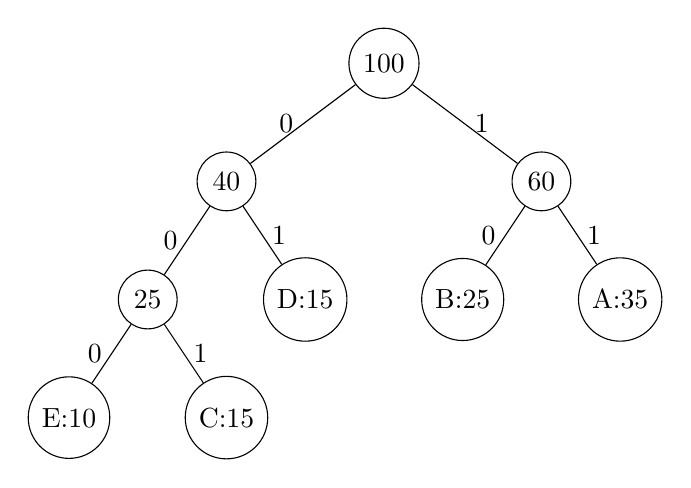
\begin{tikzpicture}[level distance=1.5cm,
level 1/.style={sibling distance=4cm},
level 2/.style={sibling distance=2cm},
level 3/.style={sibling distance=2cm}]

\node[circle,draw] {100}
    child {node[circle,draw] {40}
        child {node[circle,draw] {25}
            child {node[circle,draw] {E:10}
                edge from parent node[left] {0}}
            child {node[circle,draw] {C:15}
                edge from parent node[right] {1}}
            edge from parent node[left] {0}}
        child {node[circle,draw] {D:15}
            edge from parent node[right] {1}}
        edge from parent node[left] {0}}
    child {node[circle,draw] {60}
        child {node[circle,draw] {B:25}
            edge from parent node[left] {0}}
        child {node[circle,draw] {A:35}
            edge from parent node[right] {1}}
        edge from parent node[right] {1}};
\end{tikzpicture}
\end{center}

\textbf{编码方法:}
\begin{enumerate}
\item 规定左分支代表0,右分支代表1
\item 从根结点到每个叶子结点的路径组成该字符的编码
\item 具体编码过程:
\begin{itemize}
\item 字符A:根→右→右,编码为11
\item 字符B:根→右→左,编码为10
\item 字符C:根→左→左→右,编码为001
\item 字符D:根→左→右,编码为01
\item 字符E:根→左→左→左,编码为000
\end{itemize}
\end{enumerate}

编码结果:
\begin{center}
\begin{tabular}{|c|c|c|c|}
\hline
字符 & 频率 & 编码 & 编码长度 \\
\hline
A & 35 & 11 & 2 \\
B & 25 & 10 & 2 \\
C & 15 & 001 & 3 \\
D & 15 & 01 & 2 \\
E & 10 & 000 & 3 \\
\hline
\end{tabular}
\end{center}

\textbf{编码特点:}
\begin{itemize}
\item 频率高的字符使用较短的编码(A、B、D使用2位编码)
\item 频率低的字符使用较长的编码(C、E使用3位编码)
\item 任何字符的编码都不是另一个字符编码的前缀(前缀码性质)
\end{itemize}
\end{example}

\section{堆与优先队列}

\subsection{堆的定义与性质}

\begin{definition}[堆]
堆是具有下列性质的完全二叉树:
\begin{itemize}
\item \textbf{大根堆(最大堆)}:每个结点的值都大于或等于其左右孩子结点的值
\item \textbf{小根堆(最小堆)}:每个结点的值都小于或等于其左右孩子结点的值
\end{itemize}
\end{definition}

\textbf{堆的重要性质:}
\begin{enumerate}
\item 堆是完全二叉树,可以用数组存储,节省空间
\item 如果将堆按层序从1开始编号,则结点之间满足如下关系:
$$\text{大根堆:}\begin{cases}
k_i \geq k_{2i} \\
k_i \geq k_{2i+1}
\end{cases} \quad \text{小根堆:}\begin{cases}
k_i \leq k_{2i} \\
k_i \leq k_{2i+1}
\end{cases} \quad (1 \leq i \leq \lfloor n/2 \rfloor)$$
\item 对于编号为$i$的结点:
\begin{itemize}
\item 父结点编号:$\lfloor i/2 \rfloor$
\item 左孩子编号:$2i$
\item 右孩子编号:$2i+1$
\end{itemize}
\end{enumerate}

\textbf{堆的示例:}
\begin{center}
\begin{tikzpicture}[level distance=1.5cm,
level 1/.style={sibling distance=3cm},
level 2/.style={sibling distance=1.5cm},
level 3/.style={sibling distance=1cm}]

\node[circle,draw] {90}
    child {node[circle,draw] {80}
        child {node[circle,draw] {65}}
        child {node[circle,draw] {70}}}
    child {node[circle,draw] {85}
        child {node[circle,draw] {60}}
        child {node[circle,draw] {75}}};

\node at (0,-4) {\textbf{大根堆示例}};
\end{tikzpicture}
\quad
\begin{tikzpicture}[level distance=1.5cm,
level 1/.style={sibling distance=3cm},
level 2/.style={sibling distance=1.5cm},
level 3/.style={sibling distance=1cm}]

\node[circle,draw] {10}
    child {node[circle,draw] {20}
        child {node[circle,draw] {35}}
        child {node[circle,draw] {30}}}
    child {node[circle,draw] {15}
        child {node[circle,draw] {40}}
        child {node[circle,draw] {25}}};

\node at (0,-4) {\textbf{小根堆示例}};
\end{tikzpicture}
\end{center}

\subsection{堆的基本操作}

\subsubsection{堆的插入操作(向上调整)}

\textbf{算法思想:}
\begin{enumerate}
\item 将新元素插入到堆的末尾(保持完全二叉树性质)
\item 将新元素与其父结点比较,如果违反堆的性质则交换
\item 重复步骤2,直到满足堆的性质或到达根结点
\end{enumerate}

\begin{algorithm}[H]
\caption{堆的插入操作(大根堆)}
\begin{algorithmic}[1]
\REQUIRE 待插入元素$x$,堆数组$heap[]$,堆大小$size$
\ENSURE 维护堆的性质
\STATE $size \leftarrow size + 1$
\STATE $heap[size] \leftarrow x$
\STATE $i \leftarrow size$
\WHILE{$i > 1$ 且 $heap[i] > heap[i/2]$}
    \STATE 交换$heap[i]$和$heap[i/2]$
    \STATE $i \leftarrow i/2$
\ENDWHILE
\end{algorithmic}
\end{algorithm}

\begin{lstlisting}[caption=堆插入操作的C++实现]
void insertHeap(vector<int>& heap, int x) {
    heap.push_back(x);
    int i = heap.size() - 1;
    
    // 向上调整
    while (i > 0 && heap[i] > heap[(i-1)/2]) {
        swap(heap[i], heap[(i-1)/2]);
        i = (i-1)/2;
    }
}
\end{lstlisting}

\subsubsection{堆的删除操作(向下调整)}

\textbf{算法思想:}
\begin{enumerate}
\item 保存堆顶元素(要删除的元素)
\item 将堆的最后一个元素移到堆顶
\item 从堆顶开始向下调整,与较大的孩子交换(大根堆)
\item 重复调整直到满足堆的性质
\end{enumerate}

\begin{algorithm}[H]
\caption{堆的删除操作(大根堆)}
\begin{algorithmic}[1]
\REQUIRE 堆数组$heap[]$,堆大小$size$
\ENSURE 删除堆顶元素并维护堆的性质
\STATE $result \leftarrow heap[1]$
\STATE $heap[1] \leftarrow heap[size]$
\STATE $size \leftarrow size - 1$
\STATE $i \leftarrow 1$
\WHILE{$2i \leq size$}
    \STATE $j \leftarrow 2i$ \COMMENT{左孩子}
    \IF{$j < size$ 且 $heap[j] < heap[j+1]$}
        \STATE $j \leftarrow j+1$ \COMMENT{选择较大的孩子}
    \ENDIF
    \IF{$heap[i] \geq heap[j]$}
        \STATE \textbf{break} \COMMENT{已满足堆性质}
    \ELSE
        \STATE 交换$heap[i]$和$heap[j]$
        \STATE $i \leftarrow j$
    \ENDIF
\ENDWHILE
\RETURN $result$
\end{algorithmic}
\end{algorithm}

\subsubsection{建堆操作}

\textbf{方法一:逐个插入法}
\begin{itemize}
\item 从空堆开始,逐个插入元素
\item 时间复杂度:$O(n \log n)$
\end{itemize}

\textbf{方法二:自底向上调整法(更高效)}
\begin{itemize}
\item 将数组看作完全二叉树
\item 从最后一个非叶子结点开始,向前逐个进行向下调整
\item 时间复杂度:$O(n)$
\end{itemize}

\begin{algorithm}[H]
\caption{建堆操作(自底向上)}
\begin{algorithmic}[1]
\REQUIRE 数组$A[1..n]$
\ENSURE 将数组调整为大根堆
\FOR{$i = \lfloor n/2 \rfloor$ \textbf{downto} $1$}
    \STATE 对以$A[i]$为根的子树进行向下调整
\ENDFOR
\end{algorithmic}
\end{algorithm}

\subsection{堆排序}

\textbf{基本思想:}
\begin{enumerate}
\item 将待排序数组建成大根堆
\item 将堆顶元素(最大值)与堆的最后一个元素交换
\item 堆大小减1,对新的堆顶进行向下调整
\item 重复步骤2-3,直到堆大小为1
\end{enumerate}

\begin{lstlisting}[caption=堆排序算法实现]
void heapSort(vector<int>& arr) {
    int n = arr.size();
    
    // 建堆
    for (int i = n/2 - 1; i >= 0; i--) {
        heapify(arr, n, i);
    }
    
    // 排序
    for (int i = n-1; i > 0; i--) {
        swap(arr[0], arr[i]);  // 将最大元素放到末尾
        heapify(arr, i, 0);    // 调整剩余元素
    }
}

void heapify(vector<int>& arr, int n, int i) {
    int largest = i;
    int left = 2*i + 1;
    int right = 2*i + 2;
    
    if (left < n && arr[left] > arr[largest])
        largest = left;
    if (right < n && arr[right] > arr[largest])
        largest = right;
        
    if (largest != i) {
        swap(arr[i], arr[largest]);
        heapify(arr, n, largest);
    }
}
\end{lstlisting}

\textbf{堆排序的特点:}
\begin{itemize}
\item 时间复杂度:$O(n \log n)$(最好、平均、最坏情况都相同)
\item 空间复杂度:$O(1)$(原地排序)
\item 不稳定排序
\item 适合处理大数据量的排序问题
\end{itemize}

\subsection{优先队列}

\begin{definition}[优先队列]
优先队列是一种抽象数据类型,支持以下操作:
\begin{itemize}
\item 插入元素(insert)
\item 删除并返回优先级最高的元素(deleteMax/deleteMin)
\item 查看优先级最高的元素(top/peek)
\end{itemize}
\end{definition}

\textbf{优先队列的实现方式比较:}
\begin{center}
\begin{tabular}{|l|c|c|c|}
\hline
\textbf{实现方式} & \textbf{插入} & \textbf{删除最值} & \textbf{查找最值} \\
\hline
无序数组 & $O(1)$ & $O(n)$ & $O(n)$ \\
\hline
有序数组 & $O(n)$ & $O(1)$ & $O(1)$ \\
\hline
无序链表 & $O(1)$ & $O(n)$ & $O(n)$ \\
\hline
有序链表 & $O(n)$ & $O(1)$ & $O(1)$ \\
\hline
二叉堆 & $O(\log n)$ & $O(\log n)$ & $O(1)$ \\
\hline
\end{tabular}
\end{center}

\textbf{应用实例:}
\begin{enumerate}
\item \textbf{任务调度}:操作系统中根据优先级调度进程
\item \textbf{哈夫曼编码}:构造哈夫曼树时需要反复取出频率最小的结点
\item \textbf{图算法}:Dijkstra最短路径算法、Prim最小生成树算法
\item \textbf{事件模拟}:按时间顺序处理事件
\end{enumerate}

\begin{example}[堆操作过程演示]
对序列$(10, 20, 15, 30, 40)$建立大根堆,然后依次删除堆顶元素。

\textbf{建堆过程:}
\begin{enumerate}
\item 初始数组:$[10, 20, 15, 30, 40]$
\item 从最后一个非叶子结点开始调整($i = \lfloor 5/2 \rfloor = 2$)
\item 调整结点2(值为15):与孩子40比较,交换得到$[10, 20, 40, 30, 15]$
\item 调整结点1(值为20):与孩子30比较,交换得到$[10, 30, 40, 20, 15]$
\item 调整结点0(值为10):与孩子40比较,交换得到$[40, 30, 10, 20, 15]$
\item 继续调整:10与20比较,交换得到$[40, 30, 20, 10, 15]$
\end{enumerate}

\textbf{删除过程:}
\begin{enumerate}
\item 删除40:将15移到堆顶,调整得到$[30, 15, 20, 10]$
\item 删除30:将10移到堆顶,调整得到$[20, 15, 10]$
\item 删除20:将10移到堆顶,调整得到$[15, 10]$
\item 删除15:得到$[10]$
\item 删除10:堆为空
\end{enumerate}
\end{example}

\section{二叉树的应用}

\subsection{表达式树}

二叉表达式树是对应一个算术表达式的二叉树,具有以下特点:
\begin{enumerate}
\item 叶子结点一定是操作数
\item 分支结点一定是运算符
\end{enumerate}

\begin{example}[构造表达式树]
将表达式$(A+B) \times (C+D \times E)$转换为二叉表达式树。

\begin{center}
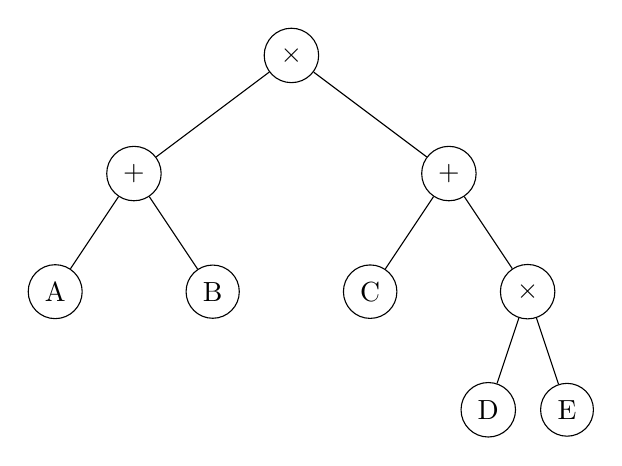
\begin{tikzpicture}[level distance=1.5cm,
level 1/.style={sibling distance=4cm},
level 2/.style={sibling distance=2cm},
level 3/.style={sibling distance=1cm}]

\node[circle,draw] {$\times$}
    child {node[circle,draw] {$+$}
        child {node[circle,draw] {A}}
        child {node[circle,draw] {B}}}
    child {node[circle,draw] {$+$}
        child {node[circle,draw] {C}}
        child {node[circle,draw] {$\times$}
            child {node[circle,draw] {D}}
            child {node[circle,draw] {E}}}};
\end{tikzpicture}
\end{center}

遍历结果:
\begin{itemize}
\item 前序遍历:$\times + A B + C \times D E$(前缀表达式)
\item 中序遍历:$A + B \times C + D \times E$(中缀表达式)
\item 后序遍历:$A B + C D E \times + \times$(后缀表达式)
\end{itemize}
\end{example}

\section{常见考点总结}

\subsection{重点掌握内容}

\begin{enumerate}
\item \textbf{二叉树的基本性质}:特别是性质1($n_0 = n_2 + 1$)和性质5(完全二叉树的编号关系)
\item \textbf{二叉树的遍历}:四种遍历方法的递归和非递归实现
\item \textbf{由遍历序列构造二叉树}:前序+中序或后序+中序唯一确定二叉树
\item \textbf{哈夫曼树的构造和编码}:算法过程和编码方法
\item \textbf{线索二叉树}:线索化过程和在线索二叉树上的遍历
\item \textbf{堆的基本操作}:插入和删除操作的调整过程
\end{enumerate}

\subsection{常见题型}

\begin{enumerate}
\item 根据二叉树的性质计算结点个数、深度等
\item 写出给定二叉树的各种遍历序列
\item 根据遍历序列构造二叉树
\item 设计二叉树遍历的递归和非递归算法
\item 哈夫曼树的构造和编码设计
\item 完全二叉树的性质和应用
\item 线索二叉树的构造和遍历
\end{enumerate}

\subsection{重要算法复杂度}

\begin{center}
\begin{tabular}{|l|c|c|}
\hline
\textbf{操作} & \textbf{时间复杂度} & \textbf{空间复杂度} \\
\hline
二叉树遍历(递归) & $O(n)$ & $O(h)$ \\
二叉树遍历(非递归) & $O(n)$ & $O(h)$ \\
哈夫曼树构造 & $O(n\log n)$ & $O(n)$ \\
堆的插入 & $O(\log n)$ & $O(1)$ \\
堆的删除 & $O(\log n)$ & $O(1)$ \\
线索化 & $O(n)$ & $O(h)$ \\
\hline
\end{tabular}
\end{center}

\section{典型例题解析}

\begin{example}[结点个数计算]
一棵完全二叉树有780个结点,其中叶子结点的个数是多少?

\textbf{解:}
设度为0、1、2的结点个数分别为$n_0$、$n_1$、$n_2$。

由二叉树性质1:$n_0 = n_2 + 1$

总结点数:$n_0 + n_1 + n_2 = 780$

对于完全二叉树,$n_1 \leq 1$(最多只有一个度为1的结点)

代入得:$(n_2 + 1) + n_1 + n_2 = 780$

即:$2n_2 + n_1 + 1 = 780$

所以:$2n_2 + n_1 = 779$

由于$n_1 \leq 1$,当$n_1 = 1$时,$n_2 = 389$,$n_0 = 390$
当$n_1 = 0$时,$n_2 = 389.5$(不是整数,不合理)

因此,叶子结点个数为390。
\end{example}

\begin{example}[遍历序列应用]
已知二叉树的前序遍历序列为ABDHECFIG,中序遍历序列为HDBECAIFG,画出该二叉树。

\textbf{解:}
\begin{enumerate}
\item 由前序序列知A是根结点
\item 由中序序列知,A左边的HDBEC是左子树,A右边的IFG是右子树
\item 递归处理左子树:前序为BDHEC,中序为HDBEC
\item 递归处理右子树:前序为FIG,中序为IFG
\end{enumerate}

最终构造的二叉树如下:

\begin{center}
\begin{tikzpicture}[level distance=1.5cm,
level 1/.style={sibling distance=5cm},
level 2/.style={sibling distance=2.5cm},
level 3/.style={sibling distance=1.5cm}]

\node[circle,draw] {A}
    child {node[circle,draw] {B}
        child {node[circle,draw] {D}
            child {node[circle,draw] {H}}
            child[missing]}
        child {node[circle,draw] {E}
            child[missing]
            child {node[circle,draw] {C}}}}
    child {node[circle,draw] {F}
        child {node[circle,draw] {I}}
        child {node[circle,draw] {G}}};
\end{tikzpicture}
\end{center}
\end{example}

\section{复习建议}

\subsection{学习方法}

\begin{enumerate}
\item \textbf{理解概念}:深入理解二叉树的定义和性质,特别是与普通树的区别
\item \textbf{掌握算法}:熟练掌握各种遍历算法的递归和非递归实现
\item \textbf{练习构造}:通过遍历序列构造二叉树的方法要反复练习
\item \textbf{应用实践}:理解二叉树在实际问题中的应用,如表达式树、哈夫曼编码等
\item \textbf{代码实现}:能够用代码实现二叉树的基本操作
\end{enumerate}

\subsection{复习重点}

\begin{enumerate}
\item 二叉树的五个基本性质及其证明和应用
\item 四种遍历方法的定义、实现和应用
\item 线索二叉树的构造和遍历
\item 哈夫曼树的构造算法和编码方法
\item 堆的定义、性质和基本操作
\item 完全二叉树的性质和应用
\end{enumerate}

\subsection{常见错误}

\begin{enumerate}
\item 混淆二叉树和度为2的树的概念
\item 遍历算法的递归出口条件错误
\item 完全二叉树性质应用错误
\item 哈夫曼编码的构造过程错误
\item 线索二叉树的线索方向搞错
\end{enumerate}

\end{document}